\chapter{Methodology and Design Process}

This chapter contains the design of the application architecture, the design of the scanning methodology and the description of the Agile method used to develop the application.

% •	Description of the application architecture suitable for security scanning (executable, terminal, later ui)
%%% o	System Settings UI and API to control every aspect of the device
% •	Agile method, stories, backlog

% IEC62443 findings and table
% Go language
% Explanation of the libraries used (Cobra for CLI, Zerolog for logging) and their benefits
% •	Design of the scanning methodology.
%%% o	Aspects covered: Outdated OS, outdated libraries (e.g., OpenSSL), outdated software, default or weak credentials, insecure network communication, …

\section{Agile method}

The \textit{Agile methodology} is a project management philosophy that involves breaking the project into phases and emphasizes continuous collaboration and improvement. Teams follow a cycle of planning, executing and evaluating. Teams choose agile so they can respond to changes in the marketplace or feedback from customers quickly without derailing a year's worth of plans. The publication of the Agile Manifesto\footnote{\url{https://agilemanifesto.org}} in 2001 marks the birth of agile as a methodology. Since then, many agile frameworks have emerged such as scrum, kanban or lean. Each embodies the core principles of frequent iteration, continuous learning and high quality in its own way.~\cite{agile-methodology} \\
We are now going to explain the Scrum framework, used by the company.

\subsection{Scrum}

Scrum is an agile project management framework, which is different from Agile, a philosophy.\\
The definition of scrum is based on empiricism and lean thinking. Empiricism says that knowledge comes from experience and that decisions are made based on what is observed. Lean thinking reduces waste and focuses on essentials. The scrum framework is heuristic; it is based on continuous learning and adjustment to fluctuating factors by acknowledging that the team does not know everything at the start of a project and it will evolve through experience. Scrum is structured to help teams to naturally adapt to changing conditions and user requirements, with re-prioritization built into the process and short release cycles so your team can constantly learn and improve.~\cite{scrum}

Scrum artefacts help to define the product, what work has to be done to create it and who has to do it. An \textit{epic} is a large body of work that can be broken down into smaller tasks. Each of these tasks is called \textit{story} and it is a short requirement written from the perspective of an end user. The story is linked to a person in the team that has to carry it out.

The two main artefacts boards are the \textit{product backlog} and the \textit{sprint backlog}. \\
The former is a list of all the tasks that need to be done; it is a dynamic list of features, requirements, improvements, fixes and epics, ordered by their priority. Essentially, it is a \textit{"To Do"} list.\\
The latter is a list of items selected for the current sprint cycle; the sprint cycle is a fixed period of time, usually up to four weeks. Before each sprint, the team selects items from the product backlog to work on. Epics are broken down into stories and stories are moved from the product backlog to the sprint backlog.~\cite{scrum-epic-stories}

\begin{figure}[t]
  \centering
  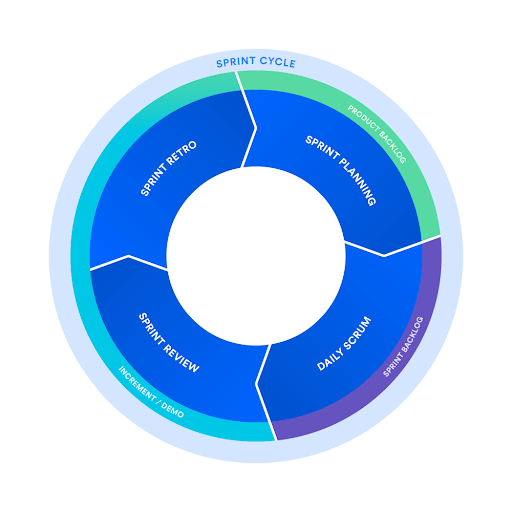
\includegraphics[width=0.8\textwidth]{chapters/04/assets/scrum}
  \caption{Scrum sprint cycle. Taken from \texttt{atlassian.com}}
  \label{fig:scrum-sprint-cycle}
\end{figure}

As visible in~\cref{fig:scrum-sprint-cycle}, Scrum is split in four principal phases:
\begin{itemize}
  \item The \textbf{sprint planning} is the initial phase of a sprint, the actual time period when the scrum team works; the team meets and decides what to do in the sprint by placing the tasks from the product backlog to the sprint backlog;
  \item The \textbf{daily scrum} is a quotidian meeting where the team members synchronize with each other. It is usually taken stand-up, as a way to not waste time and to keep the meeting short;
  \item The \textbf{sprint review} and \textbf{sprint retrospective} are the meetings at the end of the sprint where the team shows what they have done and demonstrates the work to the stakeholders and receive feedback;
\end{itemize}

The company takes advantage of the Scrum framework to manage the development of the cloud software, via the \textit{Jira} suite\footnote{\url{https://www.atlassian.com/software/jira}}, a proprietary project management tool developed by Atlassian. The tool is used to manage the product and the sprint backlog, the epics and the stories and to track the progress of the team.

% TODO: Descrivere board di Jira, colonne, priorità

Given that we were part of the office team, together with the business tutor we created a new Epic for the scanning tool and we filled it with the stories that we thought were needed to develop the tool. In this specific case, the sprint period was two months because of the internship duration. At the end of the sprint, the product backlog contained some pending stories, because of the limited time and the ongoing updating of the priorities. The daily scrum was achieved by a quotidian quick meeting with the business tutor, where we keep him updated on the progress of the stories. Of course, new stories were added to the backlog and some of them were de-prioritized.



\section{How IEC 62443 driven the design}

Recalling~\cref{sec:iec-62443}, the IEC 62443 standard provides a comprehensive framework for securing industrial control systems and operational technology networks. In order to perform a step towards the certification of the devices with the standard, the scanning tool must cover at least the aspects of the standard.

We did a case study on the standard documentation: for each of the security requirements listed in the \texttt{3-3}, \texttt{4-1} and \texttt{4-2} documents, we said:
\begin{mdframed}
  \textit{\textless\textless  Can we implement a check for this requirement in such a way as to make the user able to fix the potential issue by itself? \textgreater\textgreater}
\end{mdframed}
We considered the user as a person that has a management account on the device, and that has to interact using the settings web interface. The goal was to make the final user able to fix the reported issue without the need to update the firmware or ask for a modification on the source code or on the development lifecycle by reporting a bug report.

\cref{fig:iec62443-findings-3_3} and~\cref{fig:iec62443-findings-4_2} show the findings of the case-study. The table is divided into four columns: the first one is the security requirement title, the second one is the description text, the third is whether we believe that it is a check we should implement on a scanning tool and the fourth one contains some notes about the possible implementation.

\begin{figure}[t]
  \centering
  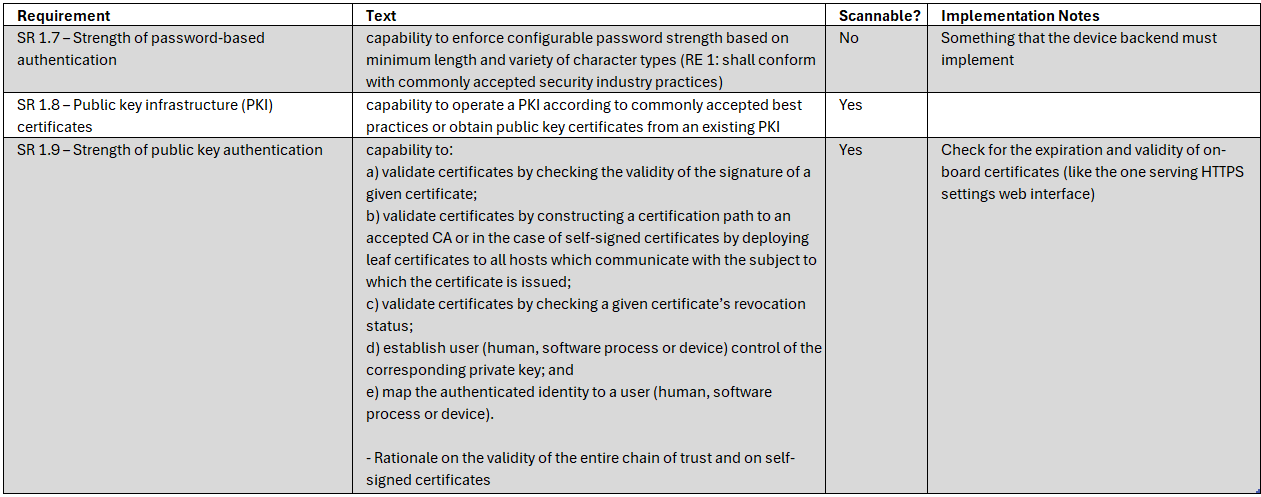
\includegraphics[width=1.0\textwidth]{chapters/04/assets/iec62443-findings-3_3}
  \caption{IEC 62443 \texttt{3-3} chosen requirements}
  \label{fig:iec62443-findings-3_3}
\end{figure}

\begin{figure}[t]
  \centering
  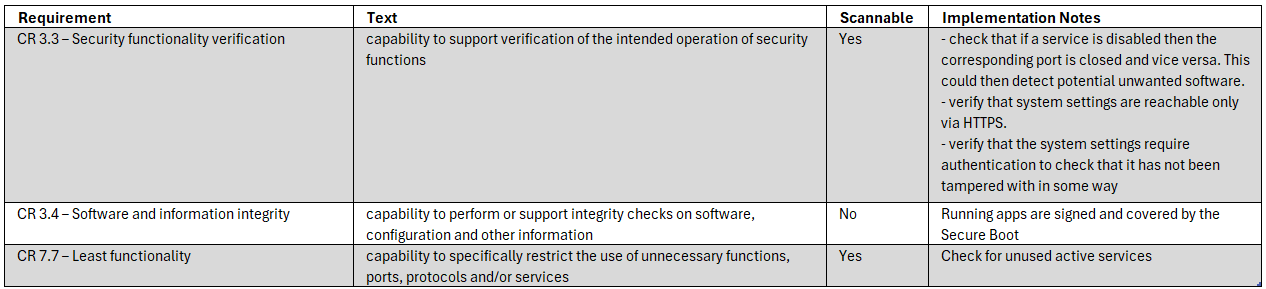
\includegraphics[width=1.0\textwidth]{chapters/04/assets/iec62443-findings-4_2}
  \caption{IEC 62443 \texttt{4-2} chosen requirements}
  \label{fig:iec62443-findings-4_2}
\end{figure}

To better explain our choices and motivations, we now take into account the \textit{SR 1.9 - Strength of public key authentication} requirement. The requirement states that there must be the capability to validate the validity of the used certificates by checking the signature, the expiration date and the revocation status. We believe that this is a check that we should implement in the scanning tool because the user can fix the issue by itself by renewing the certificate, or by changing the certificate authority related to it if needed. The implementation of the check could be done by retrieving the certificate from the device and then checking the signature, the expiration date and the revocation status. If the certificate is self-signed, the tool could suggest the user to change it with a certificate signed by a trusted certificate authority.

Instead, we now consider the \textit{SR 1.7 - Strength of password-based authentication}. The requirement states that the password must have a minimum length and a variety of character types. We put this assertion in a limbo, because if the user can set a password not respecting the requirement, the tool, which is a read-only intermediate between the user and the backend, cannot enforce the requirement. Then, the issue should be solved by the R\&D team, which should implement a password policy on the backend, and the user should be forced to change the password at the next login.

With this approach, we have identified the checks that the scanning tool should cover for sure from the standard and we have included them in the backlog of the project.

% TODO: scrum board and stories
% TODO: libraries?
